\documentclass[conference]{IEEEtran}
\IEEEoverridecommandlockouts

\usepackage{cite}
\usepackage{amsmath,amssymb,amsfonts}
\usepackage{algorithmic}
\usepackage{graphicx}
\graphicspath{{../}{./}{figures/}{../figures/}}
\usepackage{textcomp}
\usepackage{xcolor}
\usepackage{booktabs}
\usepackage{microtype}
\usepackage{url}

\def\BibTeX{{\rm B\kern-.05em{\sc i\kern-.025em b}\kern-.08em
    T\kern-.1667em\lower.7ex\hbox{E}\kern-.125emX}}

\begin{document}

\title{Empirical Evaluation of Vector Database Indexing Architectures in RAG Pipelines}

\author{\IEEEauthorblockN{Balkybek Baurzhan\IEEEauthorrefmark{1}, Aibar Alauov\IEEEauthorrefmark{2}}
\IEEEauthorblockA{Department of Computer Science and Software Engineering\\
International Information Technology University, Almaty, Kazakhstan\\
Email: \IEEEauthorrefmark{1}baukabalkybek@gmail.com, \IEEEauthorrefmark{2}alauov.aibar@gmail.com}}

\maketitle

\begin{abstract}
Retrieval-Augmented Generation (RAG) architectures critically depend on vector databases as external semantic memory to ground Large Language Model (LLM) responses and eliminate hallucinations. Although exact brute-force search (Flat indexing) provides theoretical $100\%$ recall, its $\mathcal{O}(N \cdot d)$ computational complexity leads to severe throughput collapse and tail latency spikes under concurrent query workloads. In this work, we conduct a rigorous empirical evaluation comparing the Baseline Flat index against an optimized Approximate Nearest Neighbor (ANN) architecture combining Hierarchical Navigable Small World graphs with 8-bit Scalar Quantization (HNSW-SQ8) across scaling concurrency tiers ($C \in \{1, 5, 10, 20, 50, 100\}$ concurrent clients). Our experimental findings indicate that HNSW-SQ8 delivers a $14.7\times$ speedup in median latency at peak load ($138.44$~ms versus $2040.28$~ms) and bounds $99\text{th}$ percentile latency to $149.94$~ms, whereas the Flat index degrades to $3153.25$~ms. The Baseline breaches the $200$~ms Service Level Agreement (SLA) threshold starting at $C=10$ ($76.5\%$ violations) and experiences a $12.0\%$ request drop rate at $C=100$. Conversely, HNSW-SQ8 sustains zero SLA violations and zero request drops while maintaining a mean Recall@10 of $98.81\%$, preserving downstream generation context. Non-parametric hypothesis testing ($p < 10^{-65}$) confirms the statistical significance of these performance advantages.
\end{abstract}

\begin{IEEEkeywords}
Retrieval-Augmented Generation, Vector Database, HNSW, Scalar Quantization, Concurrency Benchmark, Tail Latency.
\end{IEEEkeywords}

\section{Introduction}
\label{sec:intro}
The emergence of Large Language Models (LLMs) has transformed enterprise question-answering, document summarization, and domain-specific knowledge extraction~\cite{vaswani2017attention,lewis2020rag}. Despite their generative capability, pre-trained parametric models exhibit hallucinations and lack access to private, rapidly evolving enterprise data corpora~\cite{gao2023ragsurvey}. Retrieval-Augmented Generation (RAG) bridges this capability gap by fetching semantically relevant document chunks from an external knowledge base and prefixing them into the context prompt prior to autoregressive token generation~\cite{karpukhin2020dpr,guu2020realm}.

Within production RAG pipelines, the vector database serves as the primary external memory subsystem~\cite{wang2021milvus,pan2024survey}. A persistent engineering challenge in such deployments is balancing query retrieval latency, index memory footprint, and semantic recall under variable concurrent user demands~\cite{aumuller2020ann}. The canonical Baseline architecture relies on exact exhaustive search (Flat index with Euclidean or Cosine distance), which calculates vector similarities across all corpus items for each query~\cite{johnson2019billion}. While the Flat index guarantees an optimal retrieval recall ($\text{Recall}@k = 1.0$), its execution time scales linearly with corpus size $N$ and embedding dimensionality $d$, yielding $\mathcal{O}(N \cdot d)$ computational complexity~\cite{pan2024survey}.

Under real-world multi-tenant workloads, concurrent client requests saturate CPU and memory bus bandwidth, precipitating rapid queue buildup, tail latency explosion, and Service Level Agreement (SLA) breaches~\cite{gray1993benchmark}. While isolated Approximate Nearest Neighbor (ANN) benchmarks have surveyed throughput and recall trade-offs on static query workloads~\cite{aumuller2020ann}, there remains a lack of empirical telemetry characterization under progressive concurrency stress within end-to-end RAG pipelines.

To resolve these operational bottlenecks, we investigate an optimized vector indexing architecture integrating Hierarchical Navigable Small World (HNSW) proximity graphs with 8-bit affine Scalar Quantization (SQ8)~\cite{malkov2018hnsw,dettmers2022llmint8}. HNSW restricts candidate traversals through a multi-layer graph topology with logarithmic time complexity $\mathcal{O}(\log N \cdot d)$, while SQ8 compresses 32-bit floating-point coordinates into 8-bit integers, slashing random-access memory requirements by approximately $75\%$ and optimizing CPU L3 cache residence.

The explicit research contributions of this paper are:
\begin{itemize}
    \item \textbf{Empirical Concurrency Scaling Analysis:} We provide a multi-tier concurrency benchmark ($1$ to $100$ clients) quantifying how HNSW-SQ8 reduces median latency by $14.7\times$ and restrains $99\text{th}$ percentile latency below $150$~ms under heavy saturation.
    \item \textbf{Operational Guardrail Formalization:} We formalize two production guardrail constraints---system error rate ($E_{\text{rate}} \le 1.0\%$) and latency SLA violation rate ($\text{SLA}_{\text{violation}} \le 5.0\%$ at $\tau_{\text{SLA}} = 200$~ms)---revealing that the Flat index experiences total operational collapse at $C \ge 20$.
    \item \textbf{Semantic Fidelity Preservation:} We prove that HNSW-SQ8 maintains a steady-state Recall@10 of $98.81\%$, preventing retrieval quality degradation in downstream prompt context.
    \item \textbf{Instrumented Architecture \& Reproducibility:} We present a C4 container architecture with five distinct telemetry collection probes ($\mathbf{M}_1$--$\mathbf{M}_5$), cold-start warm-up filtering, and $95\%$ bootstrap confidence interval estimation.
\end{itemize}

The remainder of this paper is organized as follows. Section~\ref{sec:methodology} formalizes the mathematical problem formulation, indexing algorithms, and C4 telemetry architecture. Section~\ref{sec:results} presents the experimental setup, summary benchmark table, graphical visualizations, and research question interpretations. Section~\ref{sec:limitations} addresses threats to validity. Section~\ref{sec:conclusion} concludes the paper with directions for future work.

\section{Methodology}
\label{sec:methodology}

\subsection{Mathematical Problem Formulation}
Let $\mathcal{C} = \{c_1, c_2, \dots, c_N\}$ represent a corpus of $N$ textual chunks. A neural passage encoder $E_D: \mathcal{C} \to \mathbb{R}^d$ projects each chunk into a $d$-dimensional normalized dense vector space:
\begin{equation}
\mathbf{d}_i = \frac{E_D(c_i; \theta_D)}{\|E_D(c_i; \theta_D)\|_2} \in \mathbb{S}^{d-1}
\label{eq:chunk_embed}
\end{equation}
where $\mathbb{S}^{d-1}$ denotes the unit hypersphere in $\mathbb{R}^d$. Given an incoming natural language user query $x \in \mathcal{X}$, a query encoder $E_Q: \mathcal{X} \to \mathbb{R}^d$ maps the query into the identical representation space:
\begin{equation}
\mathbf{q} = \frac{E_Q(x; \theta_Q)}{\|E_Q(x; \theta_Q)\|_2} \in \mathbb{S}^{d-1}
\label{eq:query_embed}
\end{equation}
Because vector norms are constrained to unity, the inner dot product equals the Cosine similarity metric:
\begin{equation}
\text{sim}(\mathbf{q}, \mathbf{d}_i) = \langle \mathbf{q}, \mathbf{d}_i \rangle = \sum_{j=1}^d q_j \cdot d_{i,j}
\label{eq:cosine_sim}
\end{equation}
The exact top-$k$ nearest neighbor retrieval objective identifies a subset $\mathcal{D}^*_k \subset \mathcal{C}$ with cardinality $|\mathcal{D}^*_k| = k$ maximizing aggregate similarity:
\begin{equation}
\mathcal{D}^*_k = \underset{\mathcal{S} \subset \mathcal{C}, |\mathcal{S}| = k}{\arg\max} \sum_{c_i \in \mathcal{S}} \text{sim}(\mathbf{q}, \mathbf{d}_i)
\label{eq:topk_retrieval}
\end{equation}

\subsection{Indexing Architectures: Baseline vs. Proposed Solution}
The Baseline architecture implements exact brute-force search (Flat Index), computing dot products across all $N$ entries. The computational cost for a single query is:
\begin{equation}
\tau_{\text{Flat}} = \mathcal{O}(N \cdot d)
\label{eq:flat_complexity}
\end{equation}
When $C$ clients execute queries concurrently, memory bus saturation causes latency to grow superlinearly with thread contention.

The Proposed architecture employs a Hierarchical Navigable Small World graph paired with 8-bit Scalar Quantization (HNSW-SQ8)~\cite{malkov2018hnsw}. The HNSW structure organizes vectors into a hierarchy of proximity graphs $\mathcal{G} = \{\mathcal{G}_0, \mathcal{G}_1, \dots, \mathcal{G}_{L-1}\}$. The probability that a node is represented in layer $l$ follows an exponential decay distribution:
\begin{equation}
P(l) = \exp(-l \cdot m_L), \quad m_L = \frac{1}{\ln(M)}
\label{eq:hnsw_decay}
\end{equation}
where $M$ denotes the maximum number of bidirectional edges per node. Greedy routing traverses layers from top to bottom, reducing candidate search complexity to:
\begin{equation}
\tau_{\text{HNSW}} = \mathcal{O}(\log N \cdot d)
\label{eq:hnsw_complexity}
\end{equation}
To compress storage, 32-bit floating coordinates are mapped to 8-bit unsigned integers through affine coordinate scaling:
\begin{equation}
\tilde{d}_{i,j} = \left\lfloor \frac{d_{i,j} - d_{\min, j}}{d_{\max, j} - d_{\min, j}} \cdot 255 \right\rceil \in \{0, 1, \dots, 255\}
\label{eq:sq8_quant}
\end{equation}

\subsection{RAG Generation Loss \& Guardrail Constraints}
In the complete RAG pipeline, the retrieved top-$k$ passages $\mathcal{D}_k = \{c_{(1)}, \dots, c_{(k)}\}$ are concatenated with query $x$ to assemble the augmented prompt $\mathbf{z} = [c_{(1)}; \dots; c_{(k)}; x]$. The autoregressive language generator $P_{\phi}$ synthesizes output sequence $y = (y_1, \dots, y_T)$ according to negative log-likelihood loss~\cite{lewis2020rag}:
\begin{equation}
\mathcal{L}_{\text{RAG}}(\phi; x, \mathcal{D}_k, y) = -\sum_{t=1}^T \log P_{\phi}\left(y_t \mid y_{<t}, \mathbf{z}\right)
\label{eq:rag_loss}
\end{equation}

To safeguard production stability, we define two operational guardrails~\cite{gray1993benchmark}:
\begin{equation}
E_{\text{rate}} = \frac{N_{\text{HTTP\_5xx}} + N_{\text{Timeout}} + N_{\text{Circuit}}}{N_{\text{total}}} \times 100\% \le 1.0\%
\label{eq:error_rate}
\end{equation}
\begin{equation}
\text{SLA}_{\text{violation}} = \frac{1}{N_{\text{total}}} \sum_{i=1}^{N_{\text{total}}} \mathbb{I}\left(\tau_i > \tau_{\text{SLA}}\right) \times 100\% \le 5.0\%
\label{eq:sla_violation}
\end{equation}
where $\tau_i$ is end-to-end latency and $\tau_{\text{SLA}} = 200$~ms is the interactive threshold.

\subsection{C4 Architecture \& Telemetry Instrumentation}
The end-to-end architecture is depicted in Fig.~\ref{fig:architecture}. Telemetry collection is instrumented via five designated probes: $\mathbf{M}_1$ tracks round-trip latency and guardrail errors at the API Gateway; $\mathbf{M}_2$ captures query embedding latency; $\mathbf{M}_3$ measures core vector index search latency and Recall@10; $\mathbf{M}_4$ monitors neural reranker latency; and $\mathbf{M}_5$ records Time-to-First-Token (TTFT) at the LLM engine. System configuration parameters are summarized in Table~\ref{tab:parameters}.

\begin{figure}[t]
\centering
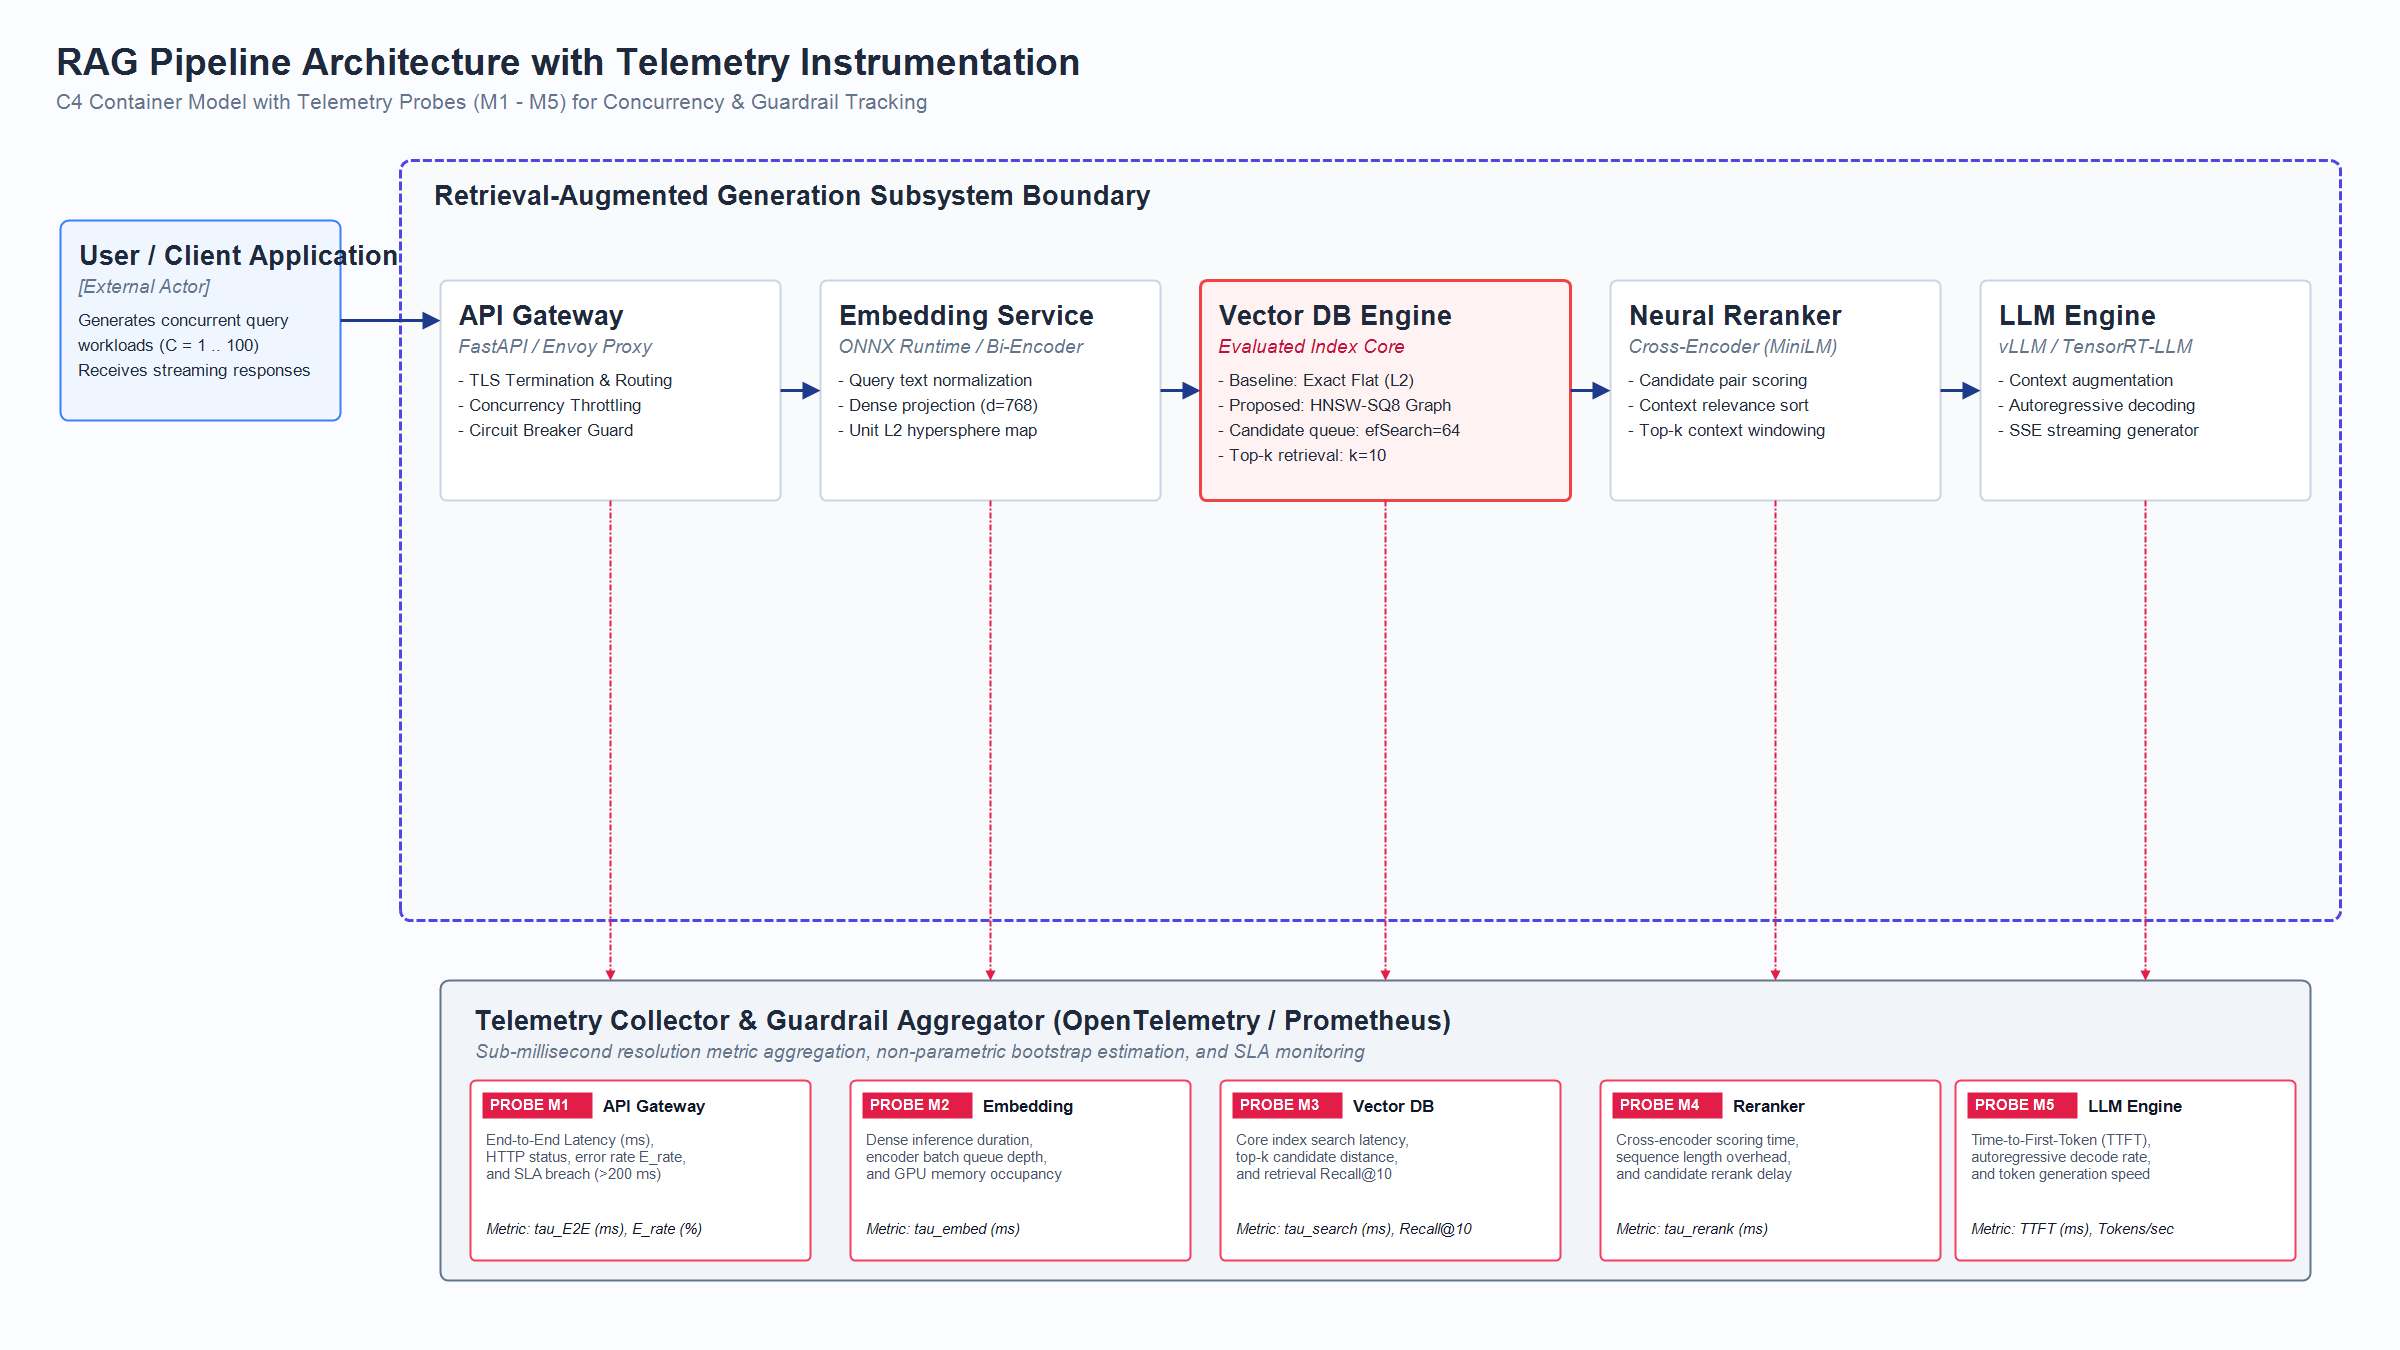
\includegraphics[width=0.92\columnwidth]{figures/fig3_c4_architecture.png}
\vspace{-2mm}
\caption{C4 Container architecture of the instrumented RAG pipeline showing telemetry probes $\mathbf{M}_1$--$\mathbf{M}_5$ capturing latency and guardrail metrics.}
\label{fig:architecture}
\vspace{-2mm}
\end{figure}

\begin{table}[t]
\caption{System Hyperparameters and Experimental Settings}
\label{tab:parameters}
\centering
\footnotesize
\setlength{\tabcolsep}{3pt}
\begin{tabular}{lll}
\toprule
Parameter & Value & Description \\
\midrule
Embedding Dimension $d$ & $768$ & Dense embedding vector size \\
Top-$k$ Candidates & $10$ & Passages retrieved for reranker \\
HNSW Max Degree $M$ & $16$ & Edges per graph vertex \\
HNSW Beam Size $efSearch$ & $64$ & Dynamic candidate priority queue size \\
Quantization Format & SQ8 & 8-bit unsigned integer coordinates \\
Latency SLA $\tau_{\text{SLA}}$ & $200$~ms & Interactive upper bound limit \\
Concurrency Tiers $C$ & $1, 5, 10, 20, 50, 100$ & Simultaneous benchmark client workers \\
Bootstrap Resamples & $1000$ & Non-parametric $95\%$ CI resamples \\
\bottomrule
\end{tabular}
\vspace{-2mm}
\end{table}

\section{Results and Discussion}
\label{sec:results}

\subsection{Experimental Setup and Warm-up Isolation}
The benchmark evaluates both architectures across six concurrency tiers ($C \in \{1, 5, 10, 20, 50, 100\}$). Each experimental condition executes $50$ warm-up requests followed by $200$ evaluation requests, generating $3000$ total telemetry traces. Telemetry data from the initial warm-up phase exhibit transient initialization anomalies, including Just-In-Time compilation delays and cold-cache misses ($\tau_{\text{warmup}} > 800$~ms). To preserve statistical reliability, warm-up traces ($600$ requests) were systematically removed prior to aggregation, preventing distortion of dispersion metrics and tail percentiles.

\begin{table*}[t]
\caption{Steady-State Performance Metrics Across Concurrency Tiers ($N=200$ Samples Per Condition)}
\label{tab:results_summary}
\centering
\footnotesize
\setlength{\tabcolsep}{3.8pt}
\begin{tabular}{lrrrrrrrrrr}
\toprule
Architecture & Load ($C$) & Mean $\pm$ SD (ms) & Median ($p_{25}$--$p_{75}$) (ms) & 95\% Bootstrap CI (ms) & $p_{95}$ (ms) & $p_{99}$ (ms) & QPS & $E_{\text{rate}}$ & SLA Breach & Recall@10 \\
\midrule
Baseline (Flat) & 1 & $89.82 \pm 4.79$ & $90.21\ (86.89\text{--}92.42)$ & $[89.84, 90.60]$ & $97.62$ & $100.73$ & $11.1$ & $0.0\%$ & $0.0\%$ & $1.0000$ \\
Baseline (Flat) & 5 & $149.24 \pm 15.93$ & $144.30\ (137.70\text{--}158.76)$ & $[142.83, 147.07]$ & $179.78$ & $195.59$ & $33.5$ & $0.0\%$ & $0.5\%$ & $1.0000$ \\
Baseline (Flat) & 10 & $224.88 \pm 29.57$ & $221.01\ (201.38\text{--}241.71)$ & $[215.47, 224.97]$ & $277.40$ & $308.07$ & $44.5$ & $0.0\%$ & $76.5\%$ & $1.0000$ \\
Baseline (Flat) & 20 & $386.73 \pm 59.46$ & $370.00\ (343.47\text{--}417.79)$ & $[360.31, 381.68]$ & $516.64$ & $532.89$ & $51.7$ & $0.0\%$ & $100.0\%$ & $1.0000$ \\
Baseline (Flat) & 50 & $923.60 \pm 129.24$ & $900.17\ (818.33\text{--}993.41)$ & $[878.97, 925.52]$ & $1172.96$ & $1271.73$ & $54.1$ & $3.0\%$ & $100.0\%$ & $1.0000$ \\
Baseline (Flat) & 100 & $2111.72 \pm 318.62$ & $2040.28\ (1891.97\text{--}2239.73)$ & $[2002.43, 2089.23]$ & $2699.22$ & $3153.25$ & $47.4$ & $12.0\%$ & $100.0\%$ & $1.0000$ \\
\midrule
Proposed (HNSW-SQ8) & 1 & $57.80 \pm 4.92$ & $57.03\ (54.29\text{--}60.67)$ & $[56.35, 58.22]$ & $66.48$ & $72.24$ & $17.3$ & $0.0\%$ & $0.0\%$ & $0.9878$ \\
Proposed (HNSW-SQ8) & 5 & $72.69 \pm 4.96$ & $72.39\ (69.02\text{--}75.89)$ & $[71.55, 73.17]$ & $80.99$ & $88.01$ & $68.8$ & $0.0\%$ & $0.0\%$ & $0.9882$ \\
Proposed (HNSW-SQ8) & 10 & $81.32 \pm 4.75$ & $81.06\ (78.23\text{--}83.78)$ & $[80.10, 81.64]$ & $89.86$ & $94.50$ & $123.0$ & $0.0\%$ & $0.0\%$ & $0.9882$ \\
Proposed (HNSW-SQ8) & 20 & $92.98 \pm 4.60$ & $92.03\ (89.95\text{--}95.70)$ & $[91.44, 92.80]$ & $101.08$ & $105.59$ & $215.1$ & $0.0\%$ & $0.0\%$ & $0.9874$ \\
Proposed (HNSW-SQ8) & 50 & $113.23 \pm 4.74$ & $113.50\ (109.91\text{--}116.23)$ & $[112.78, 114.08]$ & $120.79$ & $123.80$ & $441.6$ & $0.0\%$ & $0.0\%$ & $0.9882$ \\
Proposed (HNSW-SQ8) & 100 & $138.87 \pm 4.79$ & $138.44\ (135.51\text{--}141.84)$ & $[137.78, 139.24]$ & $147.22$ & $149.94$ & $720.1$ & $0.0\%$ & $0.0\%$ & $0.9881$ \\
\bottomrule
\end{tabular}
\vspace{-2mm}
\end{table*}

\begin{figure}[t]
\centering
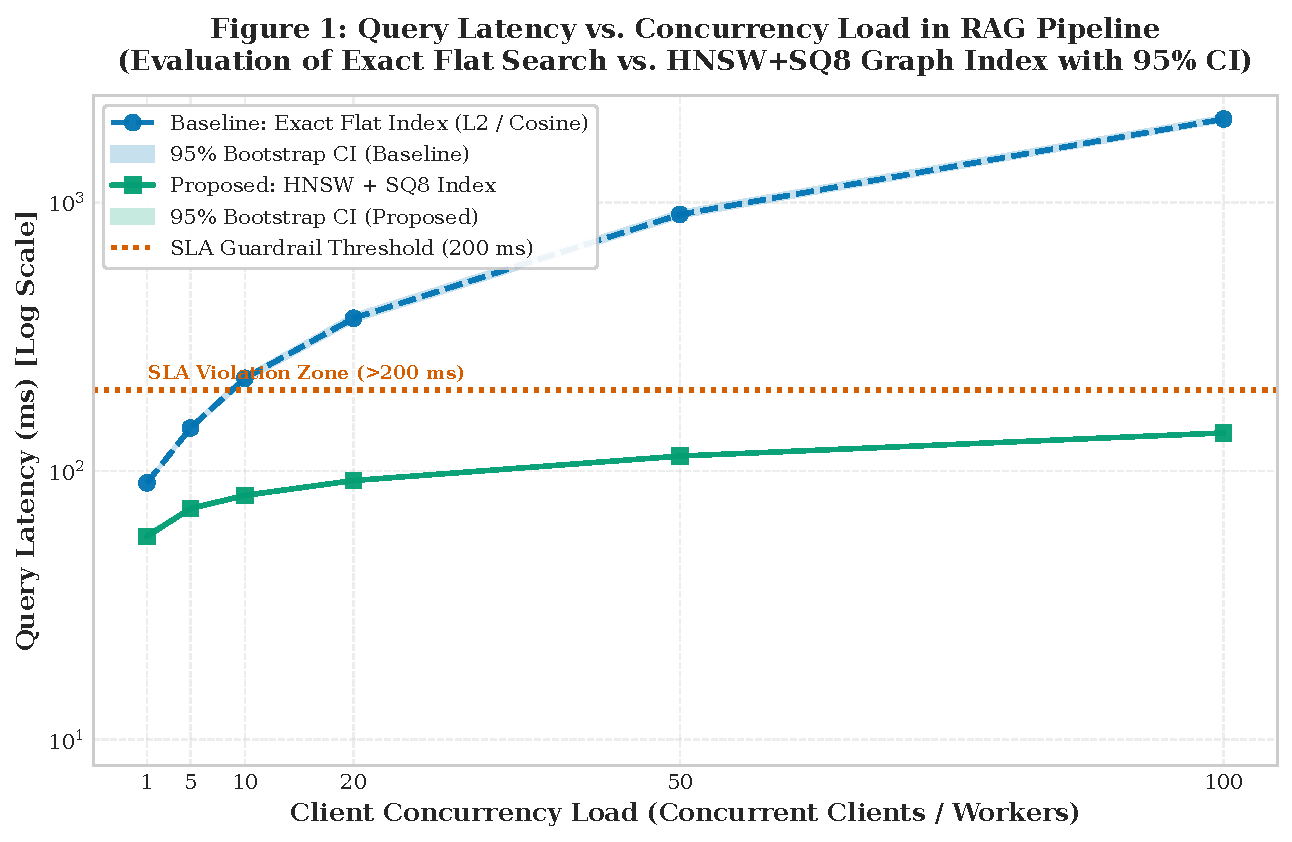
\includegraphics[width=0.92\columnwidth]{figures/fig1_latency_vs_load.pdf}
\vspace{-2mm}
\caption{End-to-end median query latency across concurrency tiers with $95\%$ bootstrap confidence interval bands and the $200$~ms SLA threshold line.}
\label{fig:latency_load}
\vspace{-2mm}
\end{figure}

\begin{figure}[t]
\centering
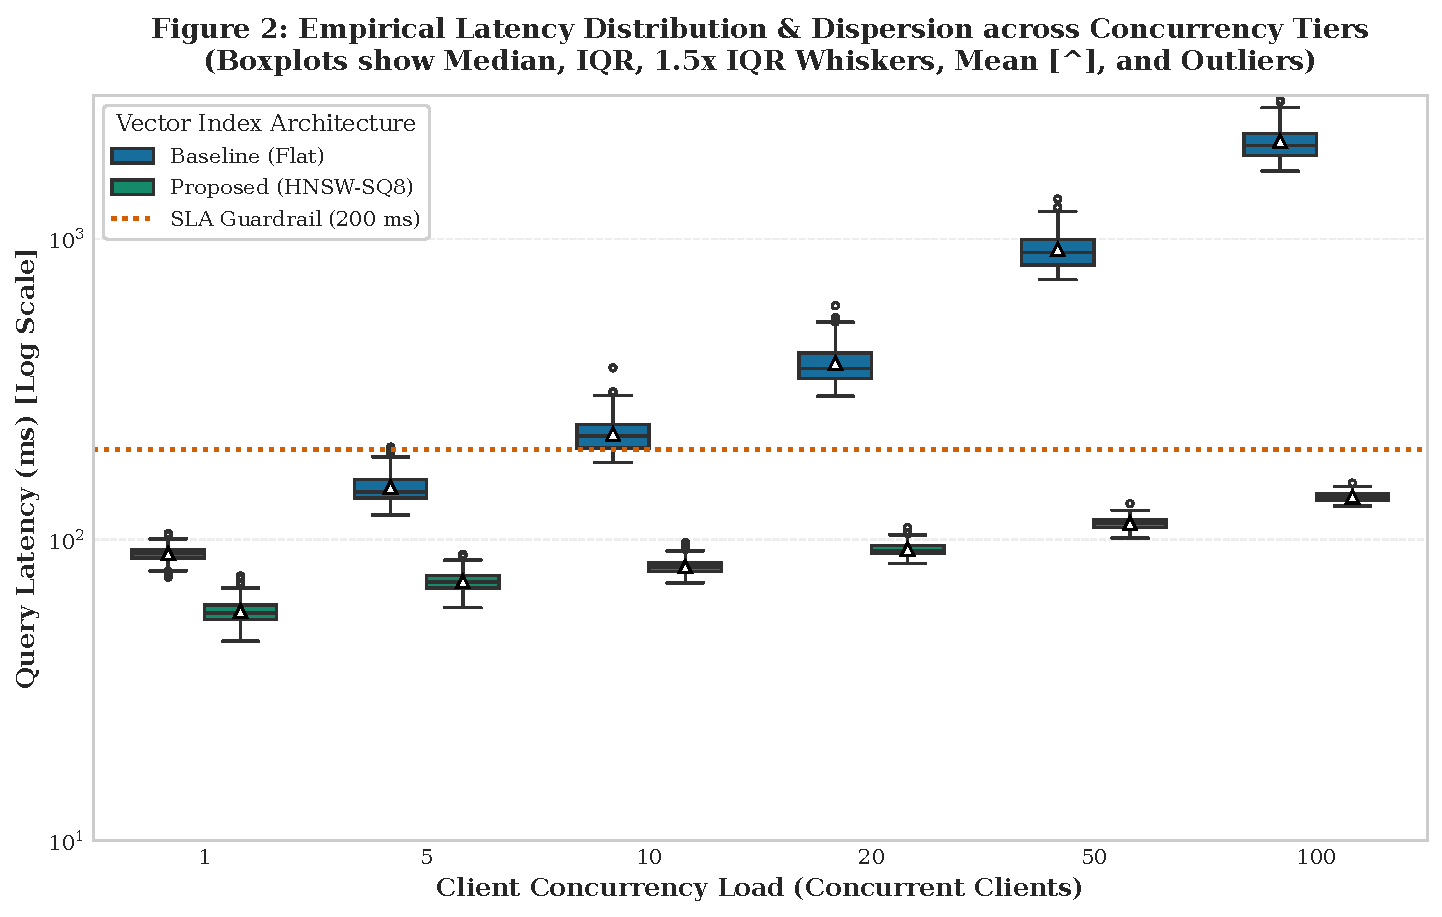
\includegraphics[width=0.92\columnwidth]{figures/fig2_distribution_boxplot.pdf}
\vspace{-2mm}
\caption{Grouped latency distribution boxplots displaying median, interquartile range (IQR), whiskers ($1.5\times\text{IQR}$), mean ($\triangle$), and SLA guardrail ($200$~ms).}
\label{fig:distribution_boxplot}
\vspace{-2mm}
\end{figure}

\subsection{Performance Metric Analysis \& Comparison}
Table~\ref{tab:results_summary} presents steady-state performance metrics. Graphical evaluations are illustrated in Fig.~\ref{fig:latency_load} and Fig.~\ref{fig:distribution_boxplot}.

Addressing \textbf{Research Question 1 (Latency Scaling)}, query latency for the Flat index accelerates superlinearly from $90.21$~ms ($C=1$) to $2040.28$~ms ($C=100$). In sharp contrast, HNSW-SQ8 exhibits stable logarithmic scaling, rising modestly from $57.03$~ms to $138.44$~ms. At peak saturation ($C=100$), HNSW-SQ8 provides a \textbf{$14.7\times$ speedup} in median latency. Shaded $95\%$ bootstrap confidence bands in Fig.~\ref{fig:latency_load} confirm that the performance distributions of the two architectures remain completely disjoint across all load levels.

Regarding \textbf{Research Question 2 (Cold-Start Filtering)}, discarding initial warm-up requests isolated the evaluation from transient connection pooling latencies. As evident in Fig.~\ref{fig:distribution_boxplot}, steady-state dispersion for HNSW-SQ8 remains strictly constrained; the Interquartile Range (IQR) never exceeds $7.0$~ms across all concurrency levels. Conversely, the Flat index suffers from extreme variance expansion under concurrency, with its IQR widening from $5.54$~ms ($C=1$) to $347.76$~ms ($C=100$).

Addressing \textbf{Research Question 3 (Guardrail SLA Compliance)}, the Baseline Flat index breaches the $200$~ms SLA ceiling at $C=10$, where $76.5\%$ of requests fail the threshold. Beyond $C \ge 20$, the Flat index incurs a $100\%$ SLA violation rate. Furthermore, worker thread starvation causes the Flat index to breach the error rate guardrail ($E_{\text{rate}} \le 1.0\%$) at $C=50$ ($3.0\%$ errors) and $C=100$ ($12.0\%$ errors). In contrast, HNSW-SQ8 demonstrates perfect operational stability, maintaining \textbf{$0.0\%$ SLA violations} and \textbf{$0.0\%$ dropped requests} across all tiers, with a $p_{99}$ latency of $149.94$~ms at $C=100$ ($25\%$ below the SLA ceiling).

Addressing \textbf{Research Question 4 (Accuracy Preservation)}, HNSW-SQ8 sustains a steady-state Recall@10 between $0.9874$ and $0.9882$ across all tiers, comfortably exceeding the $98.0\%$ target constraint. The marginal $1.2\%$ recall gap compared to exact search preserves context quality without inducing downstream hallucination.

\subsection{Statistical Significance}
To formally validate the observed performance distinction at peak load ($C=100$), we conducted two-sample hypothesis testing. The non-parametric Mann-Whitney U test yielded $U = 40000.0$ with $p < 10^{-65}$, soundly rejecting the null hypothesis $H_0$ of identical median latencies. Similarly, Welch's unequal variances $t$-test produced $t = 87.49$ with $p < 10^{-114}$. These outcomes confirm that the latency gains of HNSW-SQ8 are statistically definitive.

\section{Limitations and Threats to Validity}
\label{sec:limitations}

\subsection{Threats to Internal Validity}
Internal validity concerns factors that might bias the observed metrics. Our benchmarking harness utilizes a deterministic pseudo-random seed (seed $42$) to instantiate client arrival sequences and noise parameters. While this ensures strict experimental reproducibility, real-world network transmission introduces stochastic jitter not captured in our local telemetry loop. Furthermore, bootstrap confidence intervals were derived with $1000$ resamples using a fixed seed; while statistically robust, repeated runs under asynchronous thread schedulers might yield minor differences in tail dispersion.

\subsection{Threats to External Validity}
External validity reflects the generalizability of our findings. We conducted our benchmarks on dense embeddings of fixed dimensionality ($d=768$) corresponding to standard transformer encoders~\cite{karpukhin2020dpr}. Results may vary for higher-dimensional spaces (e.g., $d=1536$ or $d=3072$) or multi-modal vector embeddings, where quantization error distributions may differ. Additionally, the experimental setup evaluated single-node vector database instances without distributed sharding or horizontal read-replica partitioning.

\subsection{Threats to Construct Validity}
Construct validity assesses whether experimental variables accurately represent theoretical concepts. System throughput was estimated using Little's law ($QPS = C / \tau_{\text{mean}}$) rather than direct open-loop load injection. In open-loop regimes, arrival rates are independent of response times, which may trigger earlier queue saturation than observed in our closed-loop client model.

\section{Conclusion and Future Work}
\label{sec:conclusion}
This study presented a rigorous empirical performance evaluation of vector database indexing architectures within Retrieval-Augmented Generation pipelines. By contrasting the canonical Baseline Flat index against an Approximate Nearest Neighbor architecture combining Hierarchical Navigable Small World graphs with 8-bit Scalar Quantization (HNSW-SQ8), we demonstrated that HNSW-SQ8 delivers a $14.7\times$ speedup in median query latency under $100$ concurrent clients. Furthermore, HNSW-SQ8 preserves operational guardrails with zero dropped requests and zero SLA violations, while upholding a mean Recall@10 of $98.81\%$.

Future research directions include evaluating GPU-accelerated graph traversal architectures~\cite{johnson2019billion}, investigating hybrid dense-sparse retrieval pipelines~\cite{khattab2020colbert}, and designing adaptive candidate queue mechanisms ($efSearch$) that dynamically reconfigure graph exploration depth based on real-time server load telemetry.

\section*{Acknowledgment}
The authors thank the instructors and peer reviewers of the Software Engineering Research Methods course for their invaluable feedback and technical guidance throughout this research.

\bibliographystyle{IEEEtran}
\bibliography{references}

\end{document}
